\section{Auswertung}

\subsection{Energie und Wellenlänge der Cu-Kennlinien}

Die recherchierten Literaturwerte für die Energien der Kennlinien von Kupfer lauten:
\begin{align}
    E_{\alpha} = 8.046 \text{keV} \\
    E_{\beta} = 8.903 \text{keV}
\end{align}

\noindent Diese lassen sich als Differenz der Energieniveaus darstellen. Die Energieniveaus von Kupfer sind in der folgenden Grafik nocheinmal aufgetragen.

\begin{figure}[H]
    \centering
    \includegraphics{"Copper_K_Rontgen.png"}
\end{figure}
\url{https://en.wikipedia.org/wiki/File:Copper_K_Rontgen.png}

Daraus lassen sich Literaturwerte für die Wellenlängen bestimmen. Die Formel für dieses Vorhaben ist:
\begin{displaymath}
    \lambda = \frac{hc}{E}
\end{displaymath}

Mit h = 4.136$\cdot 10^{-15}$eV, c = 3$\cdot 10^{8} \frac{m}{s}$ und den oben angegebenen Daten umgerechnet in eV, ergeben sich folgende Wellenlängen:
\begin{align}
    \lambda_{\alpha} = 1.5421\cdot 10^{-10} \text{m} \nonumber \\
    \lambda_{\beta} = 1.3937\cdot 10^{-10} \text{m} \nonumber
\end{align}

\subsection{Emissionsspektrum der Röntgenröhre}

Für das Emissionsspektrum wurden für verschiedene Einfallswinkel die Impulse gemessen, die pro 10s vom Geiger-Müller-Zählrohr erfasst wurden. Daraus ergeben sich die in Tabelle \ref{tab:1} zu sehenden Daten. Diese wurden bereits auf Impulse/s angepasst. Ziel ist es nun die K\textsubscript{$\alpha$} und K\textsubscript{$\beta$} Linie zu bestimmen. Dafür werden die bereits erwähnten Daten in einem geeigneten Diagramm dargestellt. Dieses sieht wie folgt aus:

\begin{figure}[H]
    \centering
    \includegraphics{"a1.png"}
\end{figure}

\noindent An den bereits markierten Stellen sind die Kennlinien zu sehen. Dabei ist der Wert für den Winkel für die K\textsubscript{$\alpha$}-Linie = 22.6$\pm$0.2$^\circ$  und für die K\textsubscript{$\beta$}-Linie = 20.3$\pm$0.2$^\circ$.  Mit diesen Winkeln und der Bragg'schen Bedingung:
\begin{equation} \label{lambda}
    2d \sin(\alpha) = n\lambda 
\end{equation}

\noindent lassen sich nun die Wellenlängen für die beiden Kennlinien bestimmen. Die Rechnung mit d = 2.014$\cdot 10^{-10}$m liefert folgende Ergebnisse:
\begin{align}
    \lambda_{\alpha} = (1.548 \pm 0.013) \cdot 10^{-10} \text{m} \nonumber \\
    \lambda_{\beta} = (1.397 \pm 0.013) \cdot 10^{-10} \text{m} \nonumber
\end{align}

Nun können mit diesen Wellenlängen widerum die Energien berechnet werden. Dafür wird die Formel:
\begin{displaymath}
    E = \frac{h*c}{\lambda} 
\end{displaymath}
mit dem Planckschen Wirkungsquantum h = 4.136$\cdot 10^{-15}$ eV und der Lichtgeschwindigkeit c = 3$\cdot 10^{8}$. Die Energien ergeben sich damit zu:
\begin{align}
    E_{alpha} = (8.02 \pm 0.07) \cdot 10^{3} eV \nonumber \\
    E_{beta} = (8.88 \pm 0.08) \cdot 10^{3} eV \nonumber
\end{align}

\subsection{Bestimmung der Transmission als Funktion der Wellenlänge}

Die Messwerte zu dieser Messung sind in Tabelle \ref{tab:2} und \ref{tab:3} zu finden. In der Tabelle sind die gemessenen Impulse bereits auf eine Rate pro Sekunde angepasst. Diese Werte haben eine Poisson verteilte Unsicherheit. Deshalb wurden die Ursprünglich gemessenen Werte wiederhergestellt, indem sie mit der Integrationszeit von 200s multipliziert wurden. Dann wurde die Unsicherheit bestimmt und dann wurden die Werte mit der Unsicherheit wieder durch die Integrationszeit geteilt um die gewünschte Zählrate wieder herzustellen.
Anschließend wurde mit der Formel \ref{tot} eine Totzeitkorrektur der Daten vorgenommen. 
Danach ließ sich mit:
\begin{displaymath}
    T=\frac{I_{Al}}{I_0}
\end{displaymath}
\noindent die Transmission bestimmen. Um nun ein $\lambda$-T Diagramm zu erhalten erhalten werden die Wellenlängen mit den gegebenen Winkeln und \ref{lambda} bestimmt.
Dann sieht das Diagramm folgendermaßen aus:
\begin{figure}[H]
    \centering
    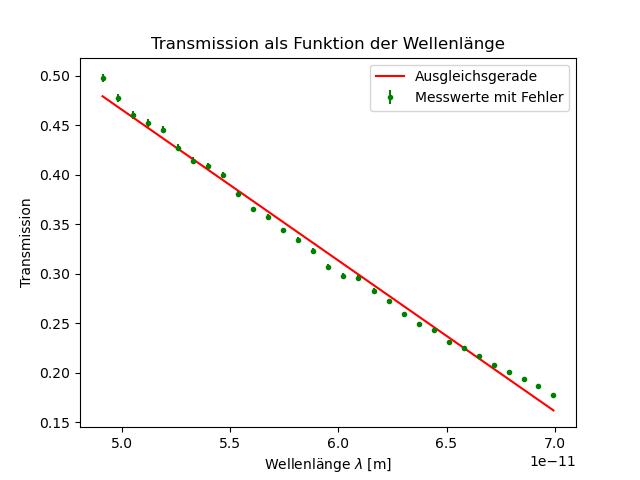
\includegraphics{Transmission.png}
\end{figure}

Für die Ausgleichsgerade wurde eine Ausgleichsrechnung mit einer Funktion der Form:
\begin{displaymath}
    T = a * \lambda + b
\end{displaymath}

\noindent durchgeführt. Die Ausgleichsrechnung mit der scipy.optimze Funktion curvefit liefert:
\begin{align}
    a = (-15194.73 \pm 239.10) \cdot 10^6 \nonumber \\
    b = 1.225 \pm 0.014 \nonumber 
\end{align}

\subsection{Bestimmung der Compton Wellenlänge}

Zur Bestimmung der Compton Wellenge wurden 3 Transmissionen gemessen. I\textsubscript{0} ist die Transmission ohne Absorber, bei I\textsubscript{1} sitzt der Al-Absorber zwischen Röntgenröhre und Streuer und für I\textsubscript{2} wurde der Al-Absorber zwischen Streuer und Geiger-Müller-Zählrohr plaziert. Bei einer Integrationszeit von 300s wurden folgende Werte gemessen:
\begin{align}
    I_0 = 2731 \nonumber \\
    I_1 = 1180 \nonumber \\
    I_2 = 1024 \nonumber
\end{align}

Daraus können wieder Transmissionen bestimmt werden. Dies geschieht auf folgende Weise:
\begin{align}
    T_1 = \frac{I_1}{I_0} \nonumber \\
    T_2 = \frac{I_2}{I_0} \nonumber
\end{align}

\noindent Für T\textsubscript{1} ergibt sich 0.432 und für T\textsubscript{2} ergibt sich 0.375.

Nun muss lediglich noch die zuvor bestimmte Funktion der Transmission invertiert werden. Als Umkehrfunktion ergibt sich:
\begin{displaymath}
    \lambda = \frac{T-b}{a}
\end{displaymath}

\noindent Damit lassen sich die Wellenlängen bestimmen:
\begin{align}
    \lambda_1 = (5.22\pm 0.12)\cdot 10^{-11} \text{m} \nonumber \\
    \lambda_2 = (5.59\pm 0.13)\cdot 10^{-11} \text{m} \nonumber
\end{align}

Damit lässt sich nun die Compton Wellenlänge bestimmen:

\begin{displaymath}
    \lambda_C = \lambda_2-\lambda_1 = (3.76\pm 0.06)\cdot 10^{-12} \text{m}
\end{displaymath}

\section{Diskussion}

\subsection{Emissionsspektrum}

Die Auswertung des Emissionsspektrums lieferte für die K\textsubscript{$\alpha$}-Linie eine Energie von $E_{alpha} = (8.02 \pm 0.07) \cdot 10^{3} eV$. Der recherchierte Literaturwert beträgt $E_{\alpha} = 8.046 \text{keV}$. Damit weicht der bestimmte Wert um gerade einmal 0.32\% ab. Das ist ein Wert der unter Betrachtung gewöhnlicher zu erwartender Messfehler außergewöhnlich genau ist. Ähnliches ist bei der K\textsubscript{$\beta$} zu erkennen. Hier weicht der bestimmte Wert $E_{beta} = (8.88 \pm 0.08) \cdot 10^{3} eV$ um 0.25\% von dem Literauturwert $E_{\beta} = 8.903 \text{keV}$ ab. 
Dieses Experiment scheint in optimalen Umständen durchgeführt worden zu sein.

\subsection{Compton Wellenlänge}

Die berechnete Compton-Wellenlänge von $(3.76\pm 0.06)\cdot 10^{-12} \text{m}$ weicht hingegen sehr deutlich von dem Literaturwert $2.426\cdot 10^{-12} \text{m}$ ab.
Die relative Abweichung beträgt hier 54.99\%. Dieser Fehler ist sehr groß. Das Problem bei dieser Messung ist, dass sie über einen sehr langen Zeitraum nur eine geringe gemessene Impulszahl liefert. Es entsteht eine sehr langsame Zählrate die am Ende nicht mehr sehr viel größer als die immer vorhandene Hintergrundrate ist, die das Geiger-Müller Zählrohr aus der Umgebung wahrnimmt. Dadurch wird die Messung sehr ungenau. Das ist allerdings auch der Grund weshalb hier eine Totzeitkorrektur unnötig wird. Der Fehler der durch den langen Messzeitraum und die vorhande Untergrundrate entsteht ist so groß, dass dagegn der Fehler durch die Totzeit quasi verschwindend gering wird.


Literaturwert von \url{https://de.wikipedia.org/wiki/Compton-Effekt}
\section{Tabellen}

\begin{minipage}{\linewidth}
    \begin{table}[H]
        \centering
    \captionof{table}{Emissionsspektrum Cu-Röntgenröhre}
    \begin{tabular}{ll}
        \toprule
        Einfallswinkel [$^\circ$] & Impulse [1/s]  \\
        \midrule
        8.0	&	    323.0 \\
        8.1	&	    316.0 \\
        8.2	&	    326.0 \\
        8.3	&	    340.0 \\
        8.4	&	    335.0 \\
        8.5	&	    343.0 \\
        8.6	&	    350.0 \\
        8.7	&	    350.0 \\
        8.8	&	    366.0 \\
        8.9	&	    357.0 \\
        9.0	&	    371.0 \\
        9.1	&	    371.0 \\
        9.2	&	    372.0 \\
        9.3	&	    364.0 \\
        9.4	&	    381.0 \\
        9.5	&	    379.0 \\
        9.6	&	    393.0 \\
        9.7	&	    375.0 \\
        9.8	&	    391.0 \\
        9.9	&	    395.0 \\
        10.0&		402.0 \\
        10.1&		405.0 \\
        10.2&		390.0 \\
        10.3&		398.0 \\
        10.4&		400.0 \\
        10.5&		418.0 \\
        10.6&		401.0 \\
        10.7&		410.0 \\
        10.8&		408.0 \\
        10.9&		409.0 \\
        11.0&		414.0 \\
        11.1&		420.0 \\
        11.2&		417.0 \\
        11.3&		417.0 \\
        11.4&		409.0 \\
        11.5&		406.0 \\
        11.6&		404.0 \\
        11.7&		405.0 \\
        11.8&		400.0 \\
        11.9&		383.0 \\
        12.0&		389.0 \\
        12.1&		382.0 \\
        12.2&		372.0 \\
        12.3&		376.0 \\
        12.4&		385.0 \\
        12.5&		384.0 \\
        12.6&		382.0 \\
        12.7&		373.0 \\
        12.8&		376.0 \\
        12.9&		373.0 \\
        13.0&		375.0 \\
        13.1&		366.0 \\
        13.2&		354.0 \\
        13.3&		341.0 \\
        13.4&		326.0 \\
        13.5&		318.0 \\
        13.6&		305.0 \\
        13.7&		296.0 \\
        13.8&		286.0 \\
        13.9&		285.0 \\
        14.0&		274.0 \\
        14.1&		264.0 \\
        14.2&		266.0 \\
        14.3&		270.0 \\
        14.4&		255.0 \\
        14.5&		255.0 \\
        14.6&		260.0 \\
        14.7&		251.0 \\
        14.8&		250.0 \\
        14.9&		248.0 \\
        15.0&		253.0 \\
        15.1&		257.0 \\
        15.2&		248.0 \\
        15.3&		242.0 \\
        15.4&		249.0 \\
        15.5&		246.0 \\
        15.6&		252.0 \\
        15.7&		236.0 \\
        15.8&		234.0 \\
        15.9&		231.0 \\
        16.0&		215.0 \\
        16.1&		217.0 \\
        16.2&		227.0 \\
        16.3&		214.0 \\
        16.4&		217.0 \\
        16.5&		210.0 \\
        16.6&		211.0 \\
        16.7&		206.0 \\
        16.8&		205.0 \\
        16.9&		198.0 \\
        17.0&		203.0 \\
        17.1&		199.0 \\
        17.2&		198.0 \\
        17.3&		191.0 \\
        17.4&		192.0 \\
        17.5&		184.0 \\
        17.6&		191.0 \\
        17.7&		188.0 \\
        17.8&		181.0 \\
        17.9&		185.0 \\
        18.0&		184.0 \\
        18.1&		179.0 \\
        18.2&		180.0 \\
        18.3&		166.0 \\
        18.4&		173.0 \\
        18.5&		167.0 \\
        18.6&		169.0 \\
        18.7&		160.0 \\
        18.8&		159.0 \\
        18.9&		157.0 \\
        19.0&		149.0 \\
        19.1&		153.0 \\
        19.2&		150.0 \\
        19.3&		147.0 \\
        19.4&		150.0 \\
        19.5&		148.0 \\
        19.6&		149.0 \\
        19.7&		143.0 \\
        19.8&		153.0 \\
        19.9&		182.0 \\
        20.0&		291.0 \\
        20.1&		1127.0 \\
        20.2&		1599.0 \\
        20.3&		1533.0 \\
        20.4&		1430.0 \\
        20.5&		1267.0 \\
        20.6&		425.0 \\
        20.7&		241.0 \\
        20.8&		225.0 \\
        20.9&		192.0 \\
        21.0&		188.0 \\
        21.1&		172.0 \\
        21.2&		168.0 \\
        21.3&		169.0 \\
        21.4&		166.0 \\
        21.5&		170.0 \\
        21.6&		174.0 \\
        21.7&		164.0 \\
        21.8&		180.0 \\
        21.9&		179.0 \\
        22.0&		191.0 \\
        22.1&		232.0 \\
        22.2&		300.0 \\
        22.3&		536.0 \\
        22.4&		4128.0 \\
        22.5&		5050.0 \\
        22.6&		4750.0 \\
        22.7&		4571.0 \\
        22.8&		4097.0 \\
        22.9&		901.0 \\
        23.0&		244.0 \\
        23.1&		179.0 \\
        23.2&		151.0 \\
        23.3&		145.0 \\
        23.4&		130.0 \\
        23.5&		121.0 \\
        23.6&		126.0 \\
        23.7&		117.0 \\
        23.8&		112.0 \\
        23.9&		110.0 \\
        24.0&		105.0 \\
        24.1&		106.0 \\
        24.2&		107.0 \\
        24.3&		95.0 \\
        24.4&		94.0\\
        24.5&		100.0\\
        24.6&		91.0\\
        24.7&		85.0\\
        24.8&		88.0\\
        24.9&		83.0\\
        25.0&		85.0\\
        \bottomrule   
    \end{tabular}
    
    \label{tab:1}
\end{table}
\end{minipage}

\begin{minipage}{\linewidth}
    \begin{table}[H]
        \centering
    \captionof{table}{Transmission mit Aluminium Absorber}
    \begin{tabular}{ll}
        \toprule
        Einfallswinkel [$^\circ$] & Impulse [1/s]  \\
        \midrule
        7.0	 & 113.5 \\
        7.1	 & 112.0 \\
        7.2	 & 112.0 \\
        7.3	 & 113.5 \\
        7.4	 & 115.0 \\
        7.5	 & 113.5 \\
        7.6	 & 113.0 \\
        7.7	 & 114.5 \\
        7.8	 & 114.0 \\
        7.9	 & 112.0 \\
        8.0	 & 109.5 \\
        8.1	 & 109.0 \\
        8.2	 & 108.0 \\
        8.3	 & 106.0 \\
        8.4	 & 104.5 \\
        8.5	 & 101.5 \\
        8.6	 & 100.0 \\
        8.7	 & 100.5 \\
        8.8	 & 97.5  \\
        8.9	 & 95.0  \\
        9.0	 & 92.5  \\
        9.1	 & 89.5  \\
        9.2	 & 88.0  \\
        9.3	 & 84.5  \\
        9.4	 & 83.0  \\
        9.5	 & 81.0  \\
        9.6	 & 78.5  \\
        9.7	 & 76.0  \\
        9.8	 & 74.0  \\
        9.9	 & 72.0  \\
        10.0 & 68.5  \\
        \bottomrule   
    \end{tabular}
    
    \label{tab:2}
\end{table}
\end{minipage}

\begin{minipage}{\linewidth}
    \begin{table}[H]
        \centering
    \captionof{table}{Transmission ohne Absorber}
    \begin{tabular}{ll}
        \toprule
        Einfallswinkel [$^\circ$] & Impulse [1/s]  \\
        \midrule
        7.0	    & 226.0 \\
        7.1	    & 232.0 \\
        7.2	    & 240.5 \\
        7.3	    & 248.0 \\
        7.4	    & 255.0 \\
        7.5	    & 262.0 \\
        7.6	    & 269.0 \\
        7.7	    & 276.0 \\
        7.8	    & 281.0 \\
        7.9	    & 289.5 \\
        8.0	    & 295.0 \\
        8.1	    & 300.0 \\
        8.2	    & 308.5 \\
        8.3	    & 311.0 \\
        8.4	    & 317.0 \\
        8.5	    & 324.0 \\
        8.6	    & 328.5 \\
        8.7	    & 332.5 \\
        8.8	    & 337.0 \\
        8.9	    & 340.5 \\
        9.0	    & 348.0 \\
        9.1	    & 350.0 \\
        9.2	    & 353.0 \\
        9.3	    & 356.5 \\
        9.4	    & 359.0 \\
        9.5	    & 363.5 \\
        9.6	    & 367.0 \\
        9.7	    & 369.0 \\
        9.8	    & 370.5 \\
        9.9	    & 375.0 \\
        10.0    & 375.5 \\
        \bottomrule   
    \end{tabular}
    
    \label{tab:3}
\end{table}
\end{minipage}

